\chapter{Introducción} 

\label{cap:intro}


% \todo{Entiendo que quieres comentar la importancia de los gráficos por computador en el mundo actual. Primero te comento errores cometidos y luego te propongo soluciones:
% 1. La generación de imágenes hace referencia solo al proceso de renderizado. El área de conocimiento son los gráficos por computar, estos incluyen animación, modelado, post-proceso.
% 2. El mundo del la generaicón y tratamiento de imagenes es demasiado amplio. Tú deberías centrarlo en el campo del los gráficos 3D (aquellos en los que la imagen generada nos permite de alguna manera (claves perpetúales captar la profundidad))
% 3. Todo el mundo sabe que los gráficos 3D estan tanformando el mundo del ocio (peliculas de animación, videojuegos) y el mundo profesional (por cierto no hablaria del mundo profesional, hablaria de la cientcia, el foramción, analisis de datos, interacción hombre máquina ...). Pero en este párrafo no concretas estas aportaciones. Ocio: ciene y videojuegos, Apredizaje: gamificación, entremiento en entornos seguros. Ciencia: Visualización y análisis de datos.... 
% Solución:
% No hables de los graficos por computador. Tu tesis se enmarca en la RV. La RV utiliza los graficos por computador y muchas otras displinas. 
% Te estoy metiendo comentarios largos por si te pueden ayudar con futuras redacciones. }

Durante los últimos años, el término de \ac{RV} se ha incorporado a nuestro lenguaje cotidiano. Esto es debido a la gran penetración que están teniendo este tipo de sistemas en nuestra vida privada y, cada vez más, en distintos ámbitos profesionales. Podemos encontrar ejemplos de estas aplicaciones en sectores tan diversos como: el mundo del ocio, donde los videojuegos son el máximo exponente del uso de estas tecnologías; el campo del entrenamiento profesional, en el que la \ac{RV} permite el desarrollo de destrezas no cognitivas en entornos controlados; el ámbito científico, donde estos sistemas facilitan la compresión de datos complejos mediante el uso de entornos inmersos. Dado el gran número de campos de aplicación y de tecnologías utilizadas, no resulta fácil indicar de forma unívoca que caracteriza un aplicación de \ac{RV}. En la bibliografía, pueden encontrarse distinta definiciones del termino:

\begin{center}
    \begin{minipage}{0.9\linewidth}
        %\vspace{5pt}%margen superior de minipage
        {\small
\emph{Virtual reality is a high-end user-computer interface that
involves real-time simulation and interactions through
multiple sensorial channels.}
        }
        \begin{flushright}
            (Burdea and Coiffet, 2003: \cite{burdea2003virtual})
        \end{flushright}
        %\vspace{5pt}%margen inferior de la minipage
    \end{minipage}
    
    \begin{minipage}{0.9\linewidth}
        %\vspace{5pt}%margen superior de minipage
        {\small
\emph{VR is the science and technology required for a user
to feel present, via perceptive, cognitive and functional
immersion and interaction, in a (computer) generated
environment. }
        }
        \begin{flushright}
            (Casarin et al., 2015: \cite{kuntz2015middlevr})
        \end{flushright}
        %\vspace{5pt}%margen inferior de la minipage
    \end{minipage}
    
\end{center}
%
%\todo{1.La realidad virtual no es una subcampo del los graficos por computdor.2.En algún lugar hay que hablar de la multidisciplinaridad de este campo (ingeniería, ciencias de la computación, psicología, graficos por computador...). Puede ir despues de la definición.}
% Este comentario esta para que no sea un parrafo nuevo
Tal y como se desprende de las definiciones anteriores, las aplicaciones \ac{RV} se caracterizan por presentar al usuario un entorno virtual a través de uno o varios sentidos, permitiéndole interactuar con el mismo y generado, en él, \new{una sensación de inmersión y presencia}.\todo{No nos metemos más en estos terminos? Tengo un libro que me paso pablo, que se puede utilizar para referenciar definiciones de estos terminos, pero lo podemos dejar así} Estos objetivos imprimen a este campo un naturaleza altamente multidisciplinar. La \ac{RV} se asienta en disciplinas como la ingeniería mecánica, los gráficos por computador, la percepción, la computación de altas prestaciones... De esta forma, el desarrollo de estas aplicaciones requiere naturalmente de expertos en distintas áreas de conocimiento.  

%\todo{ojo con afirmar cosas que no estan justificadas como "inmersión completa" o "todos los sentidos"}

El auge de la \ac{RV} es evidente, pudiéndose encontrar multitud de aplicaciones en campos tan diversos como el arte, marketing, psicología, diseño y prototipado..., siendo los sectores del entrenamiento de profesionales (de muy diversa naturaleza) y del ocio son en los que más se ha desarrollado.

%\todo{1. Es importante en las 2. 2. En lugar de decir que los entrenadores virtuales son de gran importancia, di que es donde se enmarca este trabajo de tesis.3. Explica las ventajas frente a los métodos clasicos. Es en esta última, donde la \ac{RV} tiene una gran importancia ya que se ha podido comprobar que puede traer grandes beneficios en la enseñanza y aprendizaje utilizando las nuevas tecnologías de manera atractiva frente a los métodos clásicos.}
\new{Esta tesis se centrará en el ámbito de las aplicaciones de \ac{RV} con fines de entrenamiento y práctica de actividades complejas.} En muchas profesiones existen procesos que requieren destrezas no cognitivas que solo pueden adquiriese mediante la práctica, requiriéndose técnicas de entrenamiento alternativo, y especialmente, cuando la actividad entraña un riego para el profesional o para terceros. En estos casos, las aplicaciones \ac{RV} han demostrado sus grandes ventajas sobre las técnicas de entrenamiento tradicional~\cite{PATEL2017266.e7}, proporcionando un entorno seguro, repetible y variado donde el usuario puede practicar. A pesar de ello, el desarrollo e implantación de estos sistemas no esta exento de dificultades. Se deben diseñar (con la correspondiente evaluación a posteriori) de forma que las destrezas que se pretenden adquirir sean transferibles del entorno virtual al mundo real. Además, es importante garantizar que no se adquieran malos hábitos o destrezas solamente válidas en el contexto del simulador.

Uno de los campos donde los entrenadores virtuales han penetrado con más fuerza es él de la aviación \cite{lee2017flight}. Los simuladores de vuelo, son una herramienta esencial forma parte del currículum de los nuevos pilotos comerciales\cite{piloto}. Pero estas aplicaciones, no solo se usan para el entrenamiento, sino que también proporcionan una plataforma de evaluación. %\todo{Aaron intenta ser un poco más formal: Concretamente la EASA (poner en tu lista de acrónimos) establece el uso del simulardores de vuelo en curriculum de los futuros pilotos comerciales como un requisito para obtener su licencia}
\new{Concretamente, la \ac{EASA} establece el uso del simuladores de vuelo en el curriculum de los futuros pilotos comerciales como un requisito para obtener su licencia \cite{normativa}}
%\todo{Busca si es por ley y cambia la frase}.

%\todo{Aaron te lo he cambiado para que suene más formal. Cuando metas una frase léelo 2 veces para ver si puede hacer que suene mejor}
\new{Otro campo donde son evidentes los beneficios de la \ac{RV} es el de la medicina. Las prácticas quirúrgicas requieren de la manipulación mecánica de estructuras anatómicas. De este modo, el entrenamiento de dichos procedimientos se caracteriza  por tener un alto componente práctico, de cara a adquirir las destrezas no cognitivas para que esta manipulación sea efectiva y segura.}
%\del{Por otra parte, en el ámbito médico, la prácticas quirúrgicas requieren de la manipulación se encarga de la curación del paciente mediante la manipulación mecánica de las estructuras anatómicas y por ende su aprendizaje se caracteriza por un gran componente práctico.}
Dado el riesgo que suelen representar este tipo de técnicas para los pacientes, este campo está especialmente interesado en el desarrollo de nuevas metodologías que den la  posibilidad de entrenar en entornos seguros, repetibles y variados. Por este motivo, en los últimos años han proliferado trabajos académicos que proponen nuevos simuladores médicos de \ac{RV}\cite{korzeniowski2018vcsim3,cecil2017advanced}. En la actualidad, la nueva generación de simuladores quirúrgicos va encaminada en desarrollar las capacidades de aprendizaje autónomo, evaluación e implantación de estos sistemas. A pesar de ello, estas aplicaciones aun no son comunes en los currículum de las distintas especialidades médico/quirúrgicas y la implantación de este tipo de herramientas aun debe superar un gran número de retos tecnológicos, éticos y legales. A continuación, se han listado algunos de los más importantes:
\begin{itemize}
    \item \textbf{Diversidad de procedimientos:} Existen infinidad de diversos procedimientos médicos que se caracterizan por utilizar instrumental específico y trabajar en áreas y sobre estructuras anatómicas diferentes. Esta situación dificulta el desarrollo de soluciones generales.
    \item \textbf{Limitaciones en los dispositivos \ac{E/S}:} Muchas técnicas quirúrgicas requieren de la correcta interpretación de estímulos visuales, propioceptivos y táctiles. A día de hoy, los dispositivos E/S existentes están muy limitados a la hora de presentar este tipo de información al usuario. 
    \item \textbf{Simulación de fenómenos físicos complejos con tasas de refresco y latencias interactivas:} Muchas de las interacciones mecánicas que han de reproducirse a la hora de implementar determinadas soluciones donde las simulaciones no es posible realizarlas en tiempos interactivos. Además, la complejidad aumenta al añadir la diversidad de tejidos, herramientas y fenómenos naturales que deben incluirse. 
    \item \textbf{Dificultad de obtener modelos anatómicos adecuados:} En la actualidad ninguna técnica de imagen médica (\ac{US}, \ac{TC}, \ac{IRM}...) es capaz de obtener descripciones completas de un paciente\todo{buscar cita, esta dificil, otras veces no la hemos puesto, sigo buscando?}. Por otro lado, la imágenes obtenidas deben adaptarse a representaciones que puedan utilizarse durante la simulación.
\end{itemize}
%\todo{creo que los dos últimos puntos son importantes de cara a justificar objetivos}

Es importante indicar que el objeto del listado anterior no es enumerar de forma precisa las lineas de trabajo actuales en este campo, sino que se busca ayudar al lector a entender algunos de los motivos que explican por qué la \ac{RV} aun no forma parte de programa docente de la mayoría de especialidades quirúrgicas, a pesar de sus evidentes ventajas. En está tesis, se ha trabajado en proponer soluciones que alivien algunos de las problemas derivados los dos últimos puntos del listado anterior.



% \del{En este sentido, los simuladores de \ac{RV} proporcionan una importante herramienta de aprendizaje en muchos ámbitos\todo{separa en frases}, siendo el máximo exponente los simuladores de vuelo, \del{entre otros,} ya que están totalmente integrados dentro de la formación de un profesional de la aviación}\todo{La idea es que algunos entrenadores estan tan maduros que forman parte de currículum formativo de algunas profesiones. Estos simuladores proporcionan un entorno de seguro que no entraña riesgos ni personales ni materiales y fácilmente repetible. De ello surge que estos sean los aspectos más buscados en el ámbito de la medicina, dónde los simuladores han crecido de manera exponencial durante las últimas décadas.} \todo{esta bien las ideas pero mal el orden. Mal ligado con lo que cuenta en el párrafo anterior. Mas ventajas como la planficación. Esta idea tiene que esta muy desarrollada.}

% \del{
% En cuanto a los simuladores médicos, actualmente representan un gran reto en comparación con \new{otros entrenadores como}, los simuladores de vuelo o conducción, estando estos últimos más que establecidos . La gran variabilidad entre procedimientos médicos, variedad de instrumental médico y la complejidad del cuerpo humano son las variables que representan actualmente los problemas a los que se enfrentan estos tipos de simuladores.}\todo{Me parece superficial. simulación física y rendering en tiempo real. He intentado (desarrollar estas ideas.}

% \del{La utilidad de estos simuladores van más allá del simple aprendizaje del procedimiento sino que también en entrenar las habilidades no-cognitivas que son necesarias adquirir para interiorizar y generalizar el aprendizaje. Estos simuladores permiten transmitir esas habilidades del mundo virtual al mundo real.}\todo{cita. 2. Hay que garantizar que se aprende, que las destrezas adquiridas no son validad solo en el entorno del simalador, que no se adiquieren destrezas dañinas} \del{Incluso, también pueden ser usados para permitir la planificación previa de un determinado procedimiento o la evaluación de las aptitudes de los  profesionales médicos al igual que se realiza con los simuladores de vuelo.}\todo{Las ideas esta bien pero esta tratadas de forma un poco superficial y sin justificar. 2. Que se necesita para la planificación, que se necesita para la evaluación de competencias. 3. No me gustaba la estructura. Saltaba de alante atrás }

% \del{Las mejoras continuas en el rendimiento de computadores permiten cada vez más simulaciones físicas más realistas incluso, acompañadas del desarrollo de nuevos dispositivos periféricos, son por ello el principal motivo del auge de estos simuladores. Además de enfocarse en la calidad de la simulación, la comunidad científica y la industria también está centrada en ser capaces de llevar la información de pacientes reales a los simuladores, de tal forma que puedan ser utilizados datos reales en vez de modelos artificiales creados específicamente para el simulador.\todo{esta idea la has contado antes. Es importante no estar dando saltos de atrás-adelante}}


\section{Contexto}

De cara a comprender los objetivos que se plantean más adelante en el presente documento, es importante entender el contexto en el que se ha desarrollado la presente tesis. \new{ Esto será explicado en los siguientes apartados:}\del{Este contexto, se explica en los subapartados redactados a continuación:}


\subsection{El proyecto RASimAs}
\label{intro:rasimas}

Desde noviembre de 2013 hasta octubre del año 2016, el \ac{GMRV}, de la \ac{URJC}, participó activamente el proyecto \ac{RASimAs}\cite{rasimasweb} financiado por el Séptimo Programa Marco de la Unión Europea. En él participaron investigadores y profesionales de centros y empresas punteras de 10 países diferentes. El proyecto planteó como objetivo principal el desarrollo de herramientas que facilitasen el entrenamiento y la práctica de la \ac{RA}, reduciendo los riesgos para el paciente. En concreto se propusieron dos sistemas: un entrenador de \ac{RV} llamado \ac{RASim}(fig.\ref{subfig:rasim}) y un asistente que debía entrar en quirófano \ac{RAAs}(fig.\ref{subfig:raas}). Esta tesis se enmarca en el desarrollo del primer sistema.

\begin{figure}[ht]
  \centering
  \begin{subfigure}[b]{0.5\linewidth}
    \centering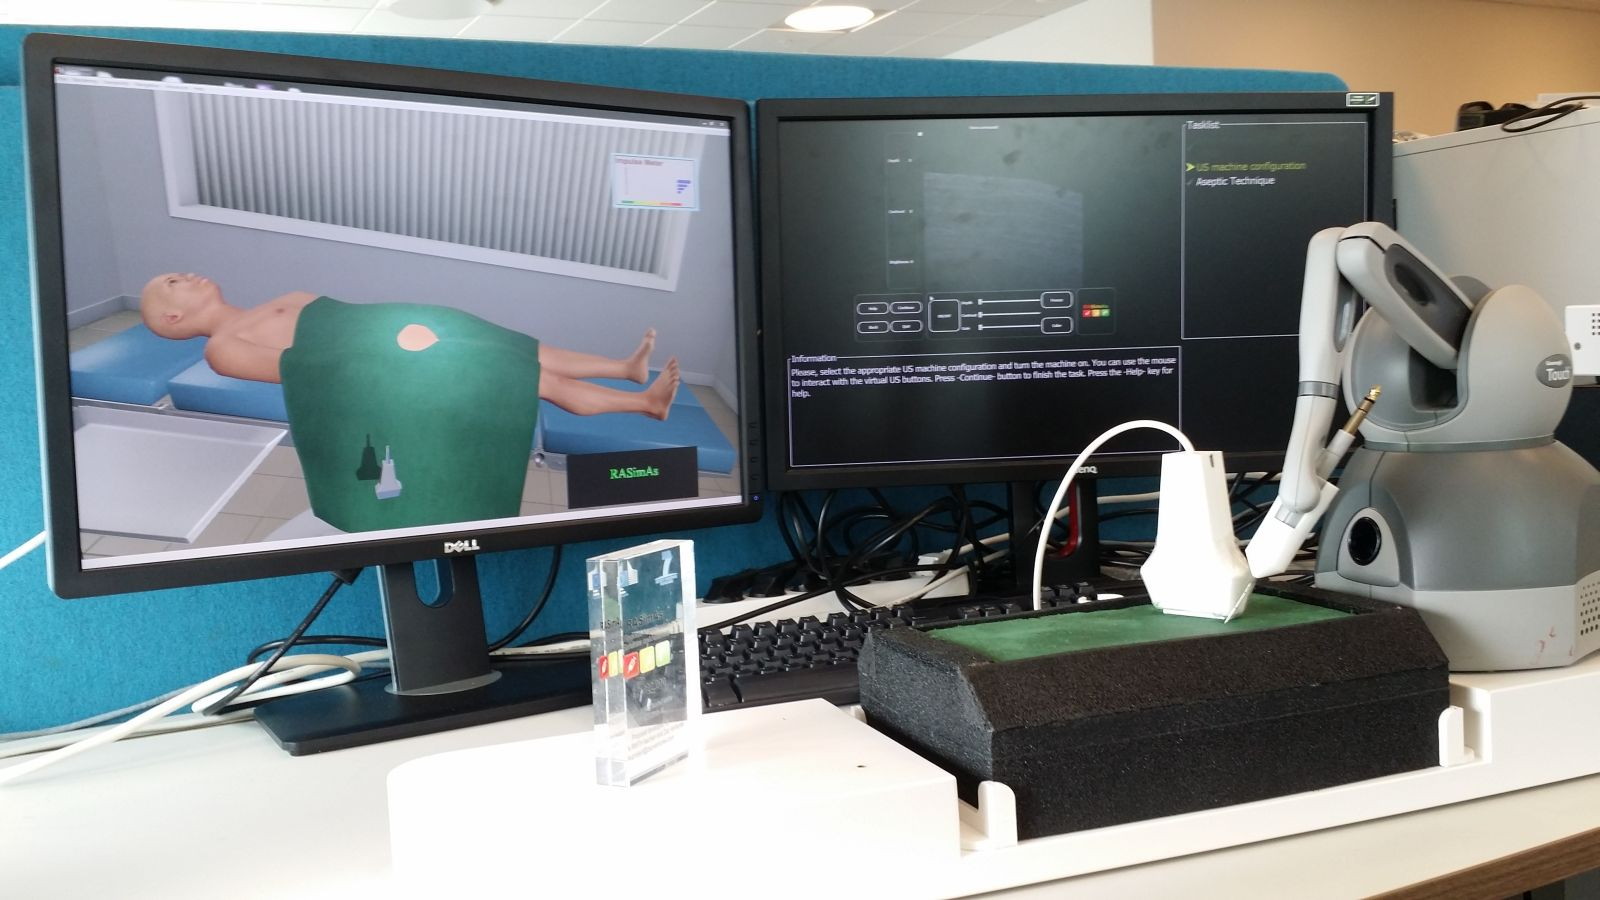
\includegraphics[width=0.9\textwidth]{IMG/sim3.jpg}
    \caption{\ac{RASim} \label{subfig:rasim}}
  \end{subfigure}%
  \begin{subfigure}[b]{0.5\linewidth}
    \centering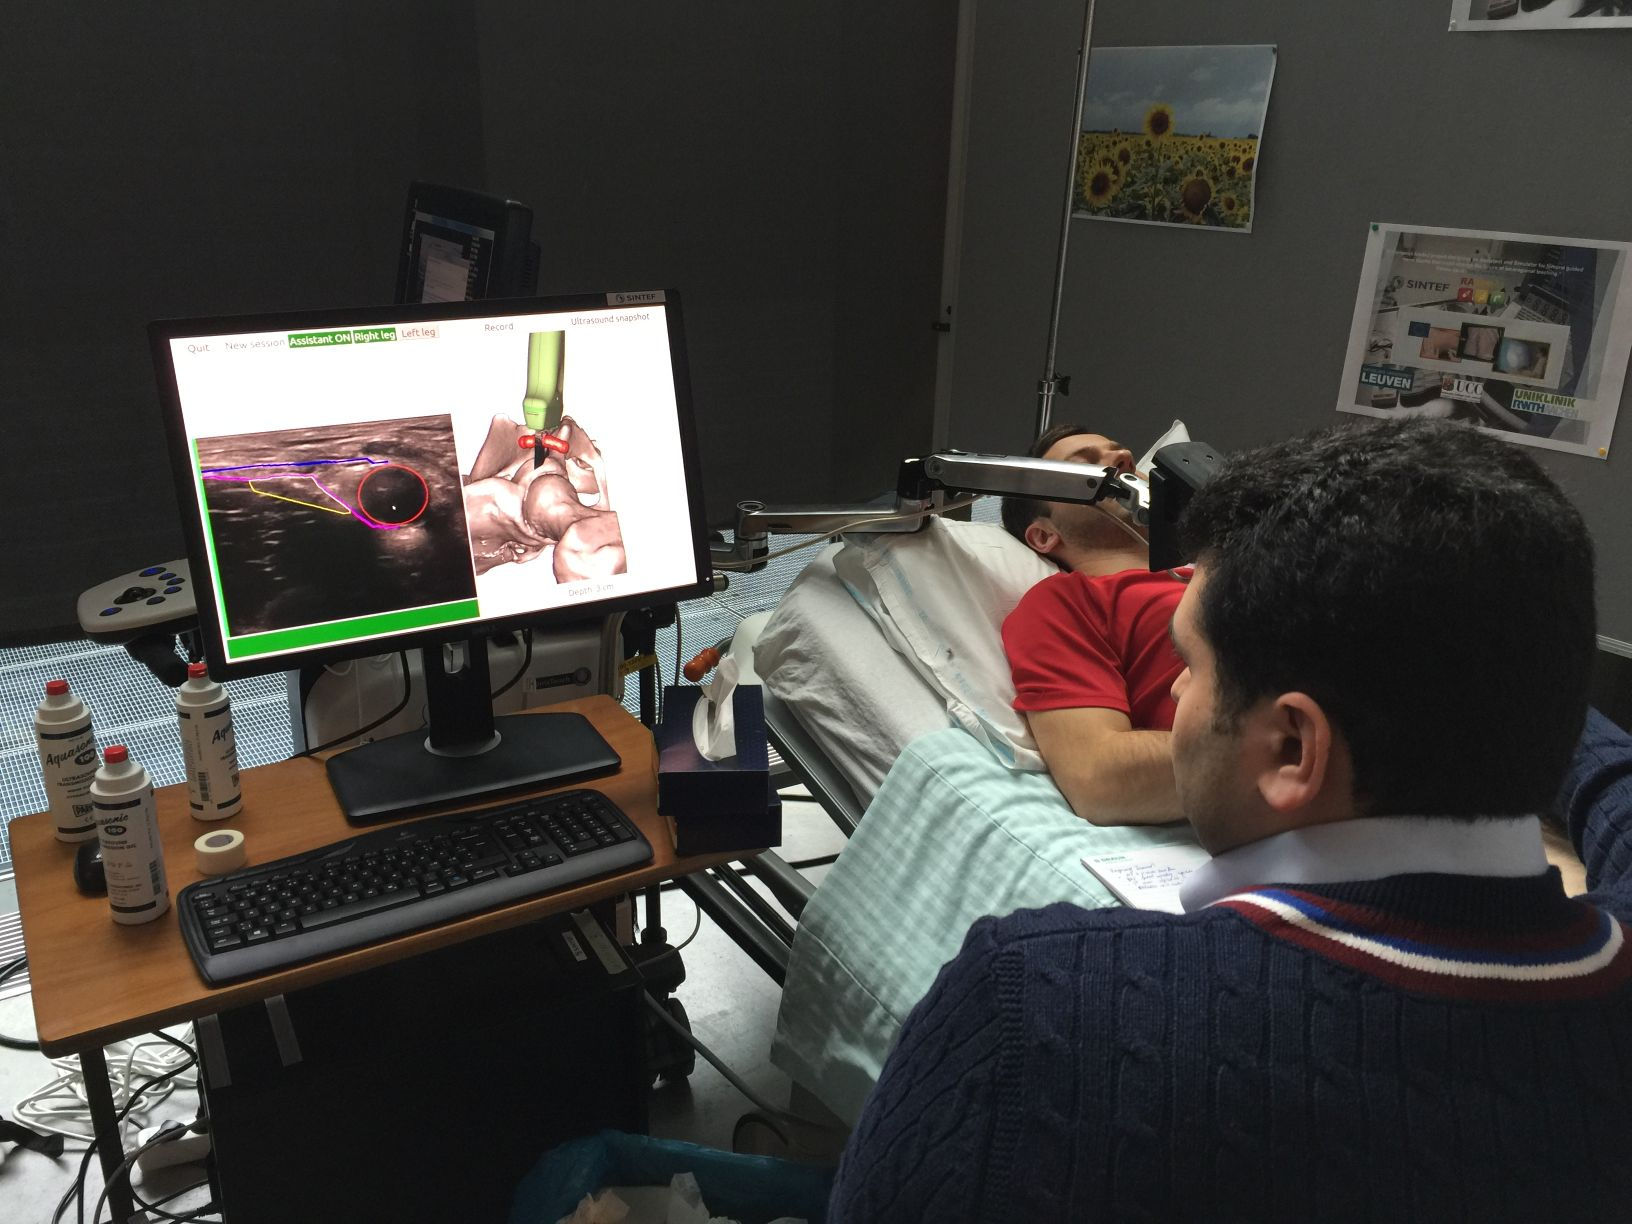
\includegraphics[width=0.9\textwidth]{IMG/raas.JPG}
    \caption{\ac{RAAs} \label{subfig:raas}}
  \end{subfigure}
  \caption{Imágenes de los prototipos desplegados de \ac{RASimAs}}
\end{figure}

%https://www.openanesthesia.org/regional-anesthesia-curriculum/
%http://rasimas.imib.rwth-aachen.de/member_area/documents_ma/Extra_Material/ISRA_Anaesthesia_Foundation_Course_Book_v1_to_print_for_ISRA_course_Oct_2_2014.pdf
%\todo{ Pon alguna cita, aquí y en el estado del arte. Por ejemplo, el CV de RA de Cork. Esto luego lo usaras en el courseware}

La \ac{RA} es un procedimiento mínimamente invasivo en el cual el médico administra un anestésico local en las proximidades del nervio que se desea bloquear \cite{CVraisra}. Esta técnica si se practica adecuadamente, frente a la anestesia general, reduce: los efectos adversos sobre el paciente, su tiempo de recuperación y el coste de la intervención \cite{PMID:26695878}. La dificultad principal del procedimiento radica en liberar el bolo anestésico alrededor del nervio, sin tocarlo, evitando liberar la dosis en el torrente sanguíneo y confirmar que esté se ha extendido correctamente a su alrededor. Actualmente existen dos técnicas para guiar la aguja a su objetivo: la estimulación eléctrica del nervio y el uso de imagen por ultrasonidos. Aunque ambas técnicas pueden combinarse, la tendencia actual es abandonar la electro-estimulación en favor del guiado por \ac{US}.

% \del{La \ac{RA} es un procedimiento médico dónde el \del{anestesiólogo}\new{anestesista!!!!!} administra anestésicos locales al paciente, a través de una aguja guiada por \ac{US} \todo{ojo hay otras formas de guiado. Tienes que ser muy preciso} en áreas cercanas a nervios específicos, produciendo una disminución de su actividad y ausencia del dolor. Esto posibilita la realización de cirugías sin necesidad de dormir al paciente completamente. De esta manera, se puede reducir el dolor postoperatorio, mejora la recuperación postoperatoria y se reduce el tiempo de hospitalización. De hecho, la anestesia regional se está imponiendo frente a la anestesia general debido a su menor coste e impacto en el paciente. \todo{cita}}
Sin embargo, esta técnica no es sencilla para los anestesistas , que no están familiarizados con la imagen por \ac{US} y requiere tener una buena base teórica y práctica  que permita a los médicos proceder de manera segura.  A día de hoy, está técnica se aprende principalmente practicándola sobre el paciente (\emph{by doing}), aunque existen otras técnicas como el uso de cadáveres\cite{Tsui2007} o \emph{fantomas}\cite{phantomra}, estas técnicas tienen limitaciones claras: alto coste, repetibilidad, aprendizaje auto-guiado, enfrentar al usuario a una amplia variabilidad anatómica... .

Por un lado, \ac{RAAs} es un sistema de guiado que superpone información adicional sobre la imagen de \ac{US}, ayudando al usuario a su identificación. El sistema dispone de \ac{tracker} y de reconocimiento de imagen que ayudan al médico a reconocer la aguja, la trayectoria de la misma y las estructuras anatómicas relevantes. 
% \del{Respecto a el sistema de guiado \ac{RAAs} consiste en asistir al anestesiólogo durante el procedimiento de \ac{RA}. Este sistema consta de unos dispositivos de seguimiento incorporados en la aguja y en la sonda del \ac{US}, de tal manera que con la información de seguimiento y la imagen de \ac{US}, el asistente proporcionará retroalimentación de inmediato que ayudará al médico a interpretar la imagen de \ac{US} de la anatomía del paciente.}
\todo{Rehaz este parrafo. 1. No entiendo porque solo destacas 2 modulos del sistema el haptico y el fantoma. No has hablado del curseware, de las métricas del modo guiado. Del modulo físico, del modulo de ultrasonidos. Estructuralo todo en partes Hw y Sw y detallalas todas. } 

\ac{RASim} es un simulador médico que recrea un entorno de \ac{RA} donde el usuario puede entrenar el procedimiento. \new{ El usuario se sitúa en frente de la mesa de trabajo donde podrá encontrar: un maniquí donde realizar el procedimiento, y los dispositivos de \ac{E/S}.
El usuario interacciona con el sistema a través de una una sonda de \ac{US}, con un \ac{tracker} magnético incorporado, y una aguja, acoplada a un dispositivo háptico. Estos dispositivos permiten al sistema seguir los movimientos del operador, y adicionalmente devolver una respuesta háptica en el caso de la aguja. El usuario puede seguir el avance del procedimiento gracias a dos pantallas. Por una parte, se genera una vista de la sala de operaciones virtual, y por otra parte, se encuentra la vista de la aplicación de entrenamiento junto con la imagen simulada de \ac{US}.
El simulador se compone de varios módulos software que se encargan de la simulación física del sistema. El usuario podrá observar como se deforman los tejidos en contacto con los instrumentos médicos, a la vez que se genera una imagen de \ac{US} necesaria para el procedimiento. 
Adicionalmente, el \ac{Courseware} convierte el simulador en una plataforma de auto-evaluación y aprendizaje. Este software dirige al usuario a través del procedimiento y gestiona todos los módulos del simulador. El usuario puede elegir entre modos de entrenamiento, donde esta aplicación registrará métricas de rendimiento con el objetivo de proporcionar retroalimentación sumativa y formativa. De esta manera, el simulador permite practicar el procedimiento completo en un entorno seguro y además mejorar sus habilidades cognitivas y no cognitivas gracias a la retroalimentación que el sistema proporciona.}

\new{ Con el objetivo de proporcionar variabilidad anatómica en el entrenamiento de los usuarios, en el proyecto \ac{RASimAs} se propuso una herramienta con la que generar una base de datos de pacientes virtuales. Este paquete de aplicaciones desarrolladas con distintos objetivos y capaces de cooperar entre sí, permiten la creación de pacientes virtuales medios que se utilizarán en \ac{RASim} y \ac{RAAs} generando las estructuras anatómicas y mecánicas necesarias de los modelos, permitiendo, adicionalmente, cambiar la postura de llegada por la posición requerida por el procedimiento.
}
%\new{Por otra parte, este mismo sistema puede ser usado como plataforma de entrenamiento autoguiado en la que el usuario puede practicar el procedimiento gracias a la retroalimentación que el sistema proporciona.}

%Se ha diseñado una mesa de trabajo donde el usuario interacciona con el sistema. En ella, se encuentran dos pantallas que sirve para proporcionar información visual al usuario. En una de ellas se puede visualizar una vista de la sala de operaciones virtual y en otra, se muestra la vista del software de entrenamiento junto con la imagen simulada de \ac{US}. En la mesa de trabajo, el usuario maneja una sonda de \ac{US}, con un \ac{tracker} magnético incorporado, y una aguja, acoplada a un dispositivo háptico, que permite al sistema el seguimiento de los movimientos del usuario. El simulador es capaz de simular la interacción y deformación de los instrumentos y tejidos, y generar una imagen de \ac{US}. El \ac{Courseware} es el encargado de dirigir al usuario a través del procedimiento y gestionar todos los modulos del simulador. 

%\todo{tienes que restructurar toda la información de RASim. 1. Objetivos (no uses la palabra objetivos todo el rato):variabilidad anatómica gran base de datos de pacientes, aprendizaje autónomo, autoevalucaion (no digas evaluación es demasiado ambicioso). 2. Modulos Hw y Sw. Importante: no me lo vuelvas a pasar hasta que lo hayas leído 3 veces. No puedo dedicar tanto tiempo a cada capítulo. Ojo Con las afirmaciones como modulo realista (si no esta evaluado, no lo sabes. Por otro lado, el módulo haptico es una mierda). }
%El objetivo de este simulador es que el usuario pueda aprender el procedimiento completo en un entorno seguro y además pueda practicar sus habilidades cognitivas y no cognitivas en el sistema. 
%\todo{demasiado ambicioso}
%de las capacidades de los profesionales, gracias a los dispositivos hápticos y a la simulación física la cual es capaz de recoger parámetros de rendimiento más allá de valoraciones subjetivas que podría tener un supervisor.\todo{No dices nada de autoguiado, ni de autoevaluación.}






%\subsection{Contribuciones al proyecto RASimAs}
%\label{intro:context}

\begin{figure}
    \centering
    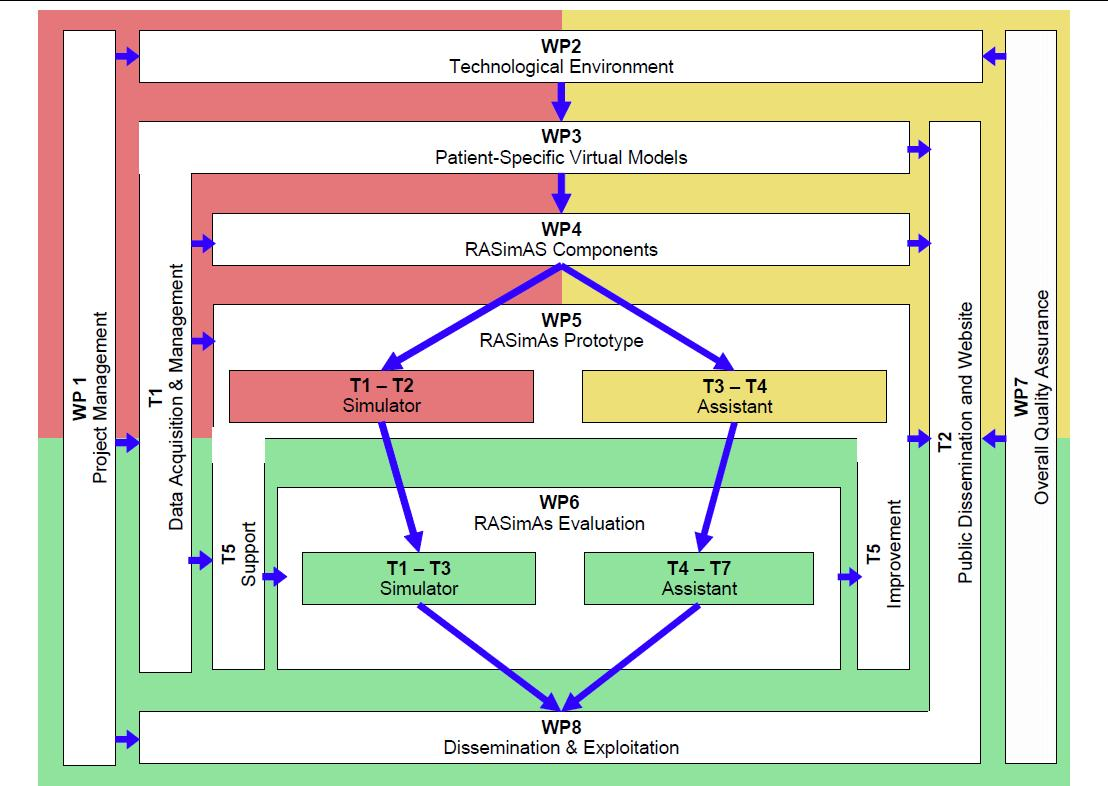
\includegraphics[width=0.95\textwidth]{IMG/wp_overview.jpg}
    \caption{División y organización de los \acl{WP} de \ac{RASimAs}}
    \label{fig:wp_rasimas}
\end{figure}
\new{
El proyecto \ac{RASimAs} se organiza en ocho \ac{WP} como se puede observar en la figura \ref{fig:wp_rasimas}. Tanto los \ac{WP} 1, 7 y 8 se encargan de la gestión, control de calidad, diseminación y explotación. El \ac{WP} 2 desarrollara la plataforma donde se integrarán todos los módulos de software y datos generados de los siguientes paquetes. En los \ac{WP} 3 y 4 se desarrollarán los componentes necesarios de los prototipos que se definen en el \ac{WP} 5. Por último, el \ac{WP} 6 se encarga de la evaluación tanto del prototipo de \ac{RASim} y como del \ac{RAAs}.  }
%\del{3. El paquete 2 se encarga del desarrollo de la plataforma en la que se integrará el sw y los datos generados. 4. El 3, 4 y 5 desarrollan los principales modulos del los dos sistemas. Son en los que hemos estado involucrados (la URJC y tu en tu tesis) y  los describiras en detalle más adelante. 5. paquete 6 evaluación del proyectoson de gestión y diseminación. }
%
%\del{Es una práctica habitual en gestión de proyectos dividir los trabajos a realizar en \ac{WP}, y estos a su vez se suelen dividir en tareas que son asignadas a cada miembro del proyecto.} 


\new{A continuación, se va a introducir brevemente los \ac{WP} 3, 4 y 5 y las tareas en las que contribuido de manera activa la \ac{URJC} y donde se localiza gran parte de la investigación realizada en esta tesis.}

\begin{itemize}
%\todo{Frase mal redactada.  No has hablado de la importancia de crear una base de datos de pacientes. Recuerda resaltar que no se buscan pacientes reales sino pacientes promedio con distinta variabilidad.}
    \item 
    \new{
El \ac{WP} 3 del proyecto \ac{RASimAs} tiene como objetivo se propone crear la herramienta \ac{TPTVPH}, \emph{un suite de aplicaciones}, que servirá para generar una base de datos de \ac{VPH} con una gran variabilidad anatómica, adecuada para conseguir un entrenamiento con modelos tipo que serán utilizados en los dos prototipos. Además, permite que el modelo pueda ser posicionado a la postura que se requiera según el procedimiento que se este realizando. Se ha dividido en las siguientes tareas:}%Este paquete se divide en seis tareas lideradas por \ac{UKA-IMI}. }
\begin{enumerate}
    \item \new{\textbf{Aquisición de datos:} Análisis y recopilación de imágenes médicas que serán utilizadas para la creación de los \ac{VPH}}
    \item \new{\textbf{Modelado anatómico:} Se realiza un registro entre las imágenes médicas y modelos anatómicos comerciales con el objetivo de generar nuevos modelos anatómicos.
    Tanto la tarea anterior como esta fueron asignadas a \ac{UKA-IMI}}
    \item \new{\textbf{Modelado mecánico:} Se generan los modelos mecánicos que se utilizarán en la simulación física del simulador. Este módulo ha sido asignado a \ac{INRIA}.}
    \item \new{\textbf{Modelado fisiológico :} En esta tarea se modelará el comportamiento físico de los tejidos cuando los nervios son electro estimulados.
    Tarea asignada a \ac{Bangor}}
    \item \new{\textbf{Herramienta de posicionamiento de pacientes:} Este módulo permite adaptar la postura de los modelos anatómicos con todos sus tejidos asociados a la pose requerida por el simulador. Tarea desarrollada en \ac{URJC}, siendo la principal línea de investigación de la presente tesis.}
    \item \new{\textbf{Integración:}
    Esta tarea asignada a \ac{FORTH}, es la encargada de hacer la integración de todos los módulos anteriores en una única herramienta ocultando los detalles técnicos a los futuros usuarios.}
\end{enumerate}
\new{Además de haber participado en las tareas asignadas a la \ac{URJC}, se ha participado activamente en la comunicación con las demás tareas, y más concretamente en la tarea de integración.}


%Uno de los módulos clave es un posicionador \todo{no inventes palabras } de pacientes que sea capaz de deformar\todo{adaptar} modelos anatómicos que contengan todo tipo de tejidos \del{externos o internos} para adecuarlos a la posición requerida por el simulador.\todo{indicar cual es la pose de partida. No has dicho en ningún momento que se usan imagenes medicas en poses determinadas. No hables de pacientes reales, habla de imagenes medicas de pacientes reales}
 %\todo{indica el numero de la tarea y di que la lideró la URJC}

\item
\new{El \ac{WP} 4 consiste en el desarrollo de los componentes necesarios de los prototipos de \ac{RASimAs}. El \ac{RASim} (Tareas 1 a 4)  y el \ac{RAAs}(Tareas 5 y 6) se han dividido en las siguientes tareas:}

\begin{enumerate}
    \item \new{\textbf{Retroalimentación háptica:}
    Desarrollo del algoritmo que permite devolver una respuesta háptica al dispositivo que simula la aguja. Esta tarea fue asignada a \ac{URJC}}
    \item \new{\textbf{Simulación física:}
    Este módulo desarrollado por \ac{INRIA} simula la deformaciones en los tejidos producidas por los instrumentos quirúrgicos.}
    \item \new{\textbf{Simulación de \ac{US}:}
    La \ac{RWTH} era la encargada de desarrollar el módulo que simulaba la generación de la imagen de \ac{US}.
    }
    \item \new{\textbf{Plataforma de entrenamiento:}
    La aplicación que se comunicaba con todos los módulos anteriores con el objetivo de proporcionar una aplicación que guiará \ac{URJC}
    }
    \item \new{\textbf{Modelado en tiempo real:} Perteneciente a \ac{RAAs}, esta tarea se basa en generar un modelo virtual a partir de las imágenes de \ac{US} que se obtienen del ecógrafo real. Con el objetivo de ayudar al usuario en la intervención.
    }
    \item \new{\textbf{Guiado en el procedimiento:}
    El asistente proporcionará ayuda al anestesista durante la intervención, ya que el sistema tiene la posición de los instrumentos y la imagen de \ac{US}.
    Tanto la tarea anterior como esta fueron asignadas a \ac{SINTEF}.
    }
\end{enumerate}
\new{La importancia de la plataforma de entrenamiento ha dado lugar a participar en las tareas 1, 2 y 3, ya que, el \ac{Courseware} se comunica y gestiona todos los módulos de \ac{RASim}.}

%\todo{Indica las tareas y en cuales has estado involucrado. Indicar cuales se han liderado.}

\item
\new{El \ac{WP} 5 se centra en el desarrollo los prototipos del simulador \ac{RASim} y el asistente \ac{RAAs}. El objetivo es crear los prototipos con intención de comprobar su validez en evaluaciones clínicas (\ac{WP} 6) con vistas a su posterior comercialización.}
\begin{itemize}
    \item \new{\textbf{Tareas 1 y 2: } Integración y construcción del prototipo \ac{RASim} a cargo de \ac{SG}. 
    }
     \item \new{\textbf{Tareas 3 y 4: } Integración y construcción del prototipo del asistente \ac{RAAs} a cargo de \ac{SINTEF}.
    }
\end{itemize}
\new{Al igual que el \ac{WP} anterior, la importancia del \ac{Courseware} en el prototipo \ac{RASim} hace que se haya trabajado conjuntamente con \ac{SG} para el desarrollo e integración de todos los módulos del simulador.}

\todo{Indica las tareas y en cuales has estado involucrado}

\end{itemize}

\subsubsection{Colaboración con la \acl{Bangor}}
\new{
Debido a la diversidad de instituciones que pueden trabajar en un proyecto de estas características, surgen relaciones entre miembros del mismo. En concreto Dr. Franck P. Vidal, miembro de la School of Computer Science de la \acl{Bangor}, ha trabajado en varios proyectos que incorporan la generación de imágenes médicas en tiempo real como \cite{villard2014interventional} y es uno de los responsables del proyecto \emph{gVirtualXRay}\cite{sujar:hal} que permite simular la generación de radiografías en tiempo real. A partir de esta tecnología y la herramienta de posicionamiento de pacientes creada para el proyecto \ac{RASimAs}, surgió la colaboración para crear un simulador de radiología diagnóstica.
%que utilizará los dos módulos para permitir a un usuario practicar el posicionamiento de un paciente por parte de un radiólogo.
La radiología es una especialidad de diagnóstico por imagen que utiliza la tecnología de los rayos X. Debido a la peligrosidad de una exposición prolongada a estos rayos, un simulador que permita al radiólogo entrenar de manera segura y utilizar el tiempo que sea necesario será de gran utilidad en el campo.
Como resultado de esta colaboración, se han podido realizar dos estancias del autor de esta tesis en la \acl{Bangor}.  }

%1. El proyecto Rasimas nos da la oportunidad de trabajar con miembros de la universidad de Bangor y conocer su trabajo.2. Frank School of Health Sciences y el otro School of Computer Science and Electronic Engineering3. Trabajan en radiologia (prescisa un poco dar mas detalles. Habla de sus publicaciones)4. Se plantea adpartar y extender las técnicas desarrolladas en el contexto de RaSimasç5. La colaboración se articula en dos estancias.}





